\documentclass{standalone}
\usepackage{tikz}
\usetikzlibrary{patterns, positioning}

\begin{document}
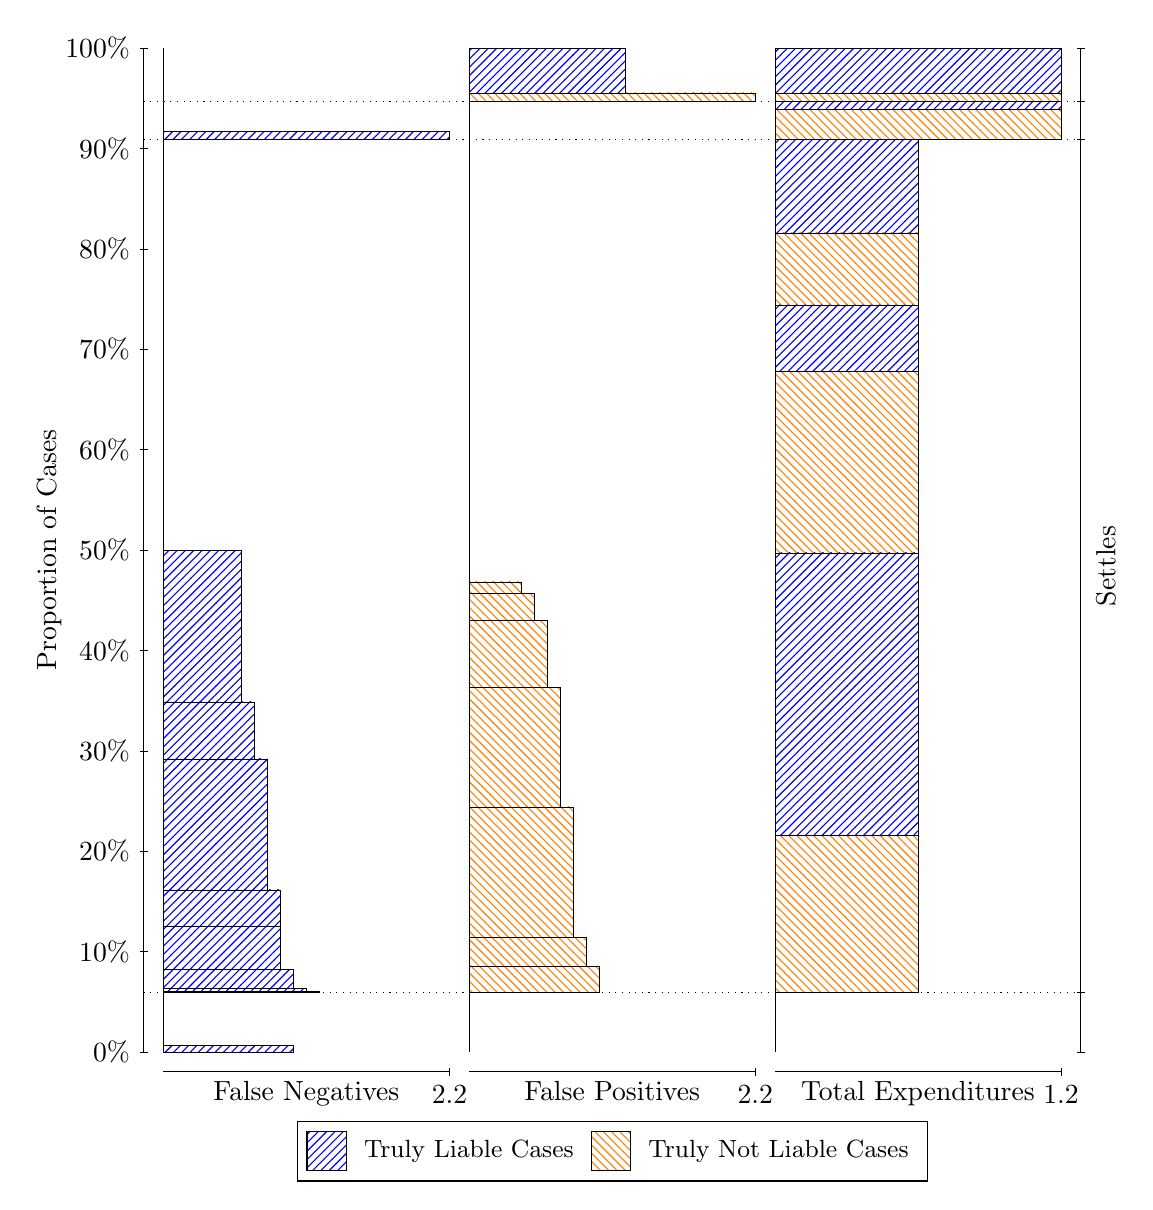
\begin{tikzpicture}
\draw[black, very thin] (1.5,1.75) -- (1.5,14.5);
\node[rotate=90, anchor=center] at (0.3, 8.125) {Proportion of Cases};
\draw[black, very thin] (1.45,1.75) -- (1.55,1.75);
\node[anchor=east] at (1.45, 1.75) {0\%};
\draw[black, very thin] (1.45,3.025) -- (1.55,3.025);
\node[anchor=east] at (1.45, 3.025) {10\%};
\draw[black, very thin] (1.45,4.3) -- (1.55,4.3);
\node[anchor=east] at (1.45, 4.3) {20\%};
\draw[black, very thin] (1.45,5.575) -- (1.55,5.575);
\node[anchor=east] at (1.45, 5.575) {30\%};
\draw[black, very thin] (1.45,6.85) -- (1.55,6.85);
\node[anchor=east] at (1.45, 6.85) {40\%};
\draw[black, very thin] (1.45,8.125) -- (1.55,8.125);
\node[anchor=east] at (1.45, 8.125) {50\%};
\draw[black, very thin] (1.45,9.4) -- (1.55,9.4);
\node[anchor=east] at (1.45, 9.4) {60\%};
\draw[black, very thin] (1.45,10.675) -- (1.55,10.675);
\node[anchor=east] at (1.45, 10.675) {70\%};
\draw[black, very thin] (1.45,11.95) -- (1.55,11.95);
\node[anchor=east] at (1.45, 11.95) {80\%};
\draw[black, very thin] (1.45,13.225) -- (1.55,13.225);
\node[anchor=east] at (1.45, 13.225) {90\%};
\draw[black, very thin] (1.45,14.5) -- (1.55,14.5);
\node[anchor=east] at (1.45, 14.5) {100\%};

\draw[black, very thin] (13.4,1.75) -- (13.4,14.5);
\draw[black, very thin] (13.35,1.75) -- (13.45,1.75);
\node[anchor=west] at (13.35, 1.75) {};
\draw[black, very thin] (13.35,2.5023) -- (13.45,2.5023);
\node[anchor=west] at (13.35, 2.5023) {};
\draw[black, very thin] (13.35,13.34) -- (13.45,13.34);
\node[anchor=west] at (13.35, 13.34) {};
\draw[black, very thin] (13.35,13.824) -- (13.45,13.824);
\node[anchor=west] at (13.35, 13.824) {};
\draw[black, very thin] (13.35,14.5) -- (13.45,14.5);
\node[anchor=west] at (13.35, 14.5) {};

\draw[black, very thin, pattern color=blue, pattern=north east lines] (1.75,1.75) rectangle (3.4015,1.8292);
\draw[black, very thin, pattern color=orange, pattern=north west lines] (1.75,1.8292) rectangle (1.75,2.5023);
\draw[black, very thin, pattern color=blue, pattern=north east lines] (1.75,2.5023) rectangle (3.7318,2.5179);
\draw[black, very thin, pattern color=blue, pattern=north east lines] (1.75,2.5179) rectangle (3.5667,2.5563);
\draw[black, very thin, pattern color=blue, pattern=north east lines] (1.75,2.5563) rectangle (3.4015,2.7962);
\draw[black, very thin, pattern color=blue, pattern=north east lines] (1.75,2.7962) rectangle (3.2364,3.3455);
\draw[black, very thin, pattern color=blue, pattern=north east lines] (1.75,3.3455) rectangle (3.2364,3.8095);
\draw[black, very thin, pattern color=blue, pattern=north east lines] (1.75,3.8095) rectangle (3.0712,5.4727);
\draw[black, very thin, pattern color=blue, pattern=north east lines] (1.75,5.4727) rectangle (2.9061,6.1958);
\draw[black, very thin, pattern color=blue, pattern=north east lines] (1.75,6.1958) rectangle (2.7409,8.1228);
\draw[black, very thin, pattern color=orange, pattern=north west lines] (1.75,8.1228) rectangle (1.75,13.34);
\draw[black, very thin, pattern color=blue, pattern=north east lines] (1.75,13.34) rectangle (5.3833,13.445);
\draw[black, very thin, pattern color=orange, pattern=north west lines] (1.75,13.445) rectangle (1.75,13.824);
\draw[black, very thin, pattern color=orange, pattern=north west lines] (1.75,13.824) rectangle (1.75,13.93);
\draw[black, very thin, pattern color=blue, pattern=north east lines] (1.75,13.93) rectangle (1.75,14.5);
\draw[black, very thin, pattern color=orange, pattern=north west lines] (5.6333,1.75) rectangle (5.6333,2.4232);
\draw[black, very thin, pattern color=blue, pattern=north east lines] (5.6333,2.4232) rectangle (5.6333,2.5023);
\draw[black, very thin, pattern color=orange, pattern=north west lines] (5.6333,2.5023) rectangle (7.2848,2.8395);
\draw[black, very thin, pattern color=orange, pattern=north west lines] (5.6333,2.8395) rectangle (7.1197,3.2065);
\draw[black, very thin, pattern color=orange, pattern=north west lines] (5.6333,3.2065) rectangle (6.9545,4.8637);
\draw[black, very thin, pattern color=orange, pattern=north west lines] (5.6333,4.8637) rectangle (6.7894,6.378);
\draw[black, very thin, pattern color=orange, pattern=north west lines] (5.6333,6.378) rectangle (6.6242,7.2279);
\draw[black, very thin, pattern color=orange, pattern=north west lines] (5.6333,7.2279) rectangle (6.4591,7.5776);
\draw[black, very thin, pattern color=orange, pattern=north west lines] (5.6333,7.5776) rectangle (6.2939,7.7192);
\draw[black, very thin, pattern color=blue, pattern=north east lines] (5.6333,7.7192) rectangle (5.6333,13.34);
\draw[black, very thin, pattern color=orange, pattern=north west lines] (5.6333,13.34) rectangle (5.6333,13.718);
\draw[black, very thin, pattern color=blue, pattern=north east lines] (5.6333,13.718) rectangle (5.6333,13.824);
\draw[black, very thin, pattern color=orange, pattern=north west lines] (5.6333,13.824) rectangle (9.2667,13.93);
\draw[black, very thin, pattern color=blue, pattern=north east lines] (5.6333,13.93) rectangle (7.6152,14.5);
\draw[black, very thin, pattern color=orange, pattern=north west lines] (9.5167,1.75) rectangle (9.5167,2.4232);
\draw[black, very thin, pattern color=blue, pattern=north east lines] (9.5167,2.4232) rectangle (9.5167,2.5023);
\draw[black, very thin, pattern color=orange, pattern=north west lines] (9.5167,2.5023) rectangle (11.333,4.4967);
\draw[black, very thin, pattern color=blue, pattern=north east lines] (9.5167,4.4967) rectangle (11.333,8.087);
\draw[black, very thin, pattern color=orange, pattern=north west lines] (9.5167,8.087) rectangle (11.333,10.396);
\draw[black, very thin, pattern color=blue, pattern=north east lines] (9.5167,10.396) rectangle (11.333,11.239);
\draw[black, very thin, pattern color=orange, pattern=north west lines] (9.5167,11.239) rectangle (11.333,12.153);
\draw[black, very thin, pattern color=blue, pattern=north east lines] (9.5167,12.153) rectangle (11.333,13.34);
\draw[black, very thin, pattern color=orange, pattern=north west lines] (9.5167,13.34) rectangle (13.15,13.718);
\draw[black, very thin, pattern color=blue, pattern=north east lines] (9.5167,13.718) rectangle (13.15,13.824);
\draw[black, very thin, pattern color=orange, pattern=north west lines] (9.5167,13.824) rectangle (13.15,13.93);
\draw[black, very thin, pattern color=blue, pattern=north east lines] (9.5167,13.93) rectangle (13.15,14.5);
\draw[black, dotted] (1.5,2.5023) -- (13.4,2.5023);
\draw[black, dotted] (1.5,13.34) -- (13.4,13.34);
\draw[black, dotted] (1.5,13.824) -- (13.4,13.824);
\draw[black, very thin] (1.75,1.5) -- (5.3833,1.5);
\node[anchor=north] at (3.5667, 1.5) {False Negatives};
\draw[black, very thin] (5.3833,1.45) -- (5.3833,1.55);
\node[anchor=north] at (5.3833, 1.45) {2.2};

\draw[black, very thin] (5.6333,1.5) -- (9.2667,1.5);
\node[anchor=north] at (7.45, 1.5) {False Positives};
\draw[black, very thin] (9.2667,1.45) -- (9.2667,1.55);
\node[anchor=north] at (9.2667, 1.45) {2.2};

\draw[black, very thin] (9.5167,1.5) -- (13.15,1.5);
\node[anchor=north] at (11.333, 1.5) {Total Expenditures};
\draw[black, very thin] (13.15,1.45) -- (13.15,1.55);
\node[anchor=north] at (13.15, 1.45) {1.2};


\node[black, centered, rotate=90] at (13.72, 7.921) {Settles};



\draw (7.449999999999999,1.5) node[draw=none] (baseCoordinate) {};
\begin{scope}[align=center]
        \matrix[scale=0.5, draw=black, below=0.5cm of baseCoordinate, nodes={draw}, column sep=0.1cm]{
            \node[rectangle, draw, minimum width=0.5cm, minimum height=0.5cm, pattern=north east lines, pattern color=blue] {}; &
            \node[draw=none, font=\small] (B) {Truly Liable Cases}; &
            \node[rectangle, draw, minimum width=0.5cm, minimum height=0.5cm, pattern=north west lines, pattern color=orange] {}; &
            \node[draw=none, font=\small] (B) {Truly Not Liable Cases}; \\
            };
\end{scope}

\end{tikzpicture}
\end{document}